\chapter[INTRODUCCIÓN HISTÓRICA DEL DODECAFONISMO]{INTRODUCCIÓN HISTÓRICA DEL DODECAFONISMO}\label{ch:historia}
	\section{Richard Wagner y la emancipación de la disonancia}
		\begin{wrapfigure}{r}{0.3\textwidth}
			\captionsetup{justification=centering, font=footnotesize}
			\vspace{-\bigskipamount}
			\centering{
			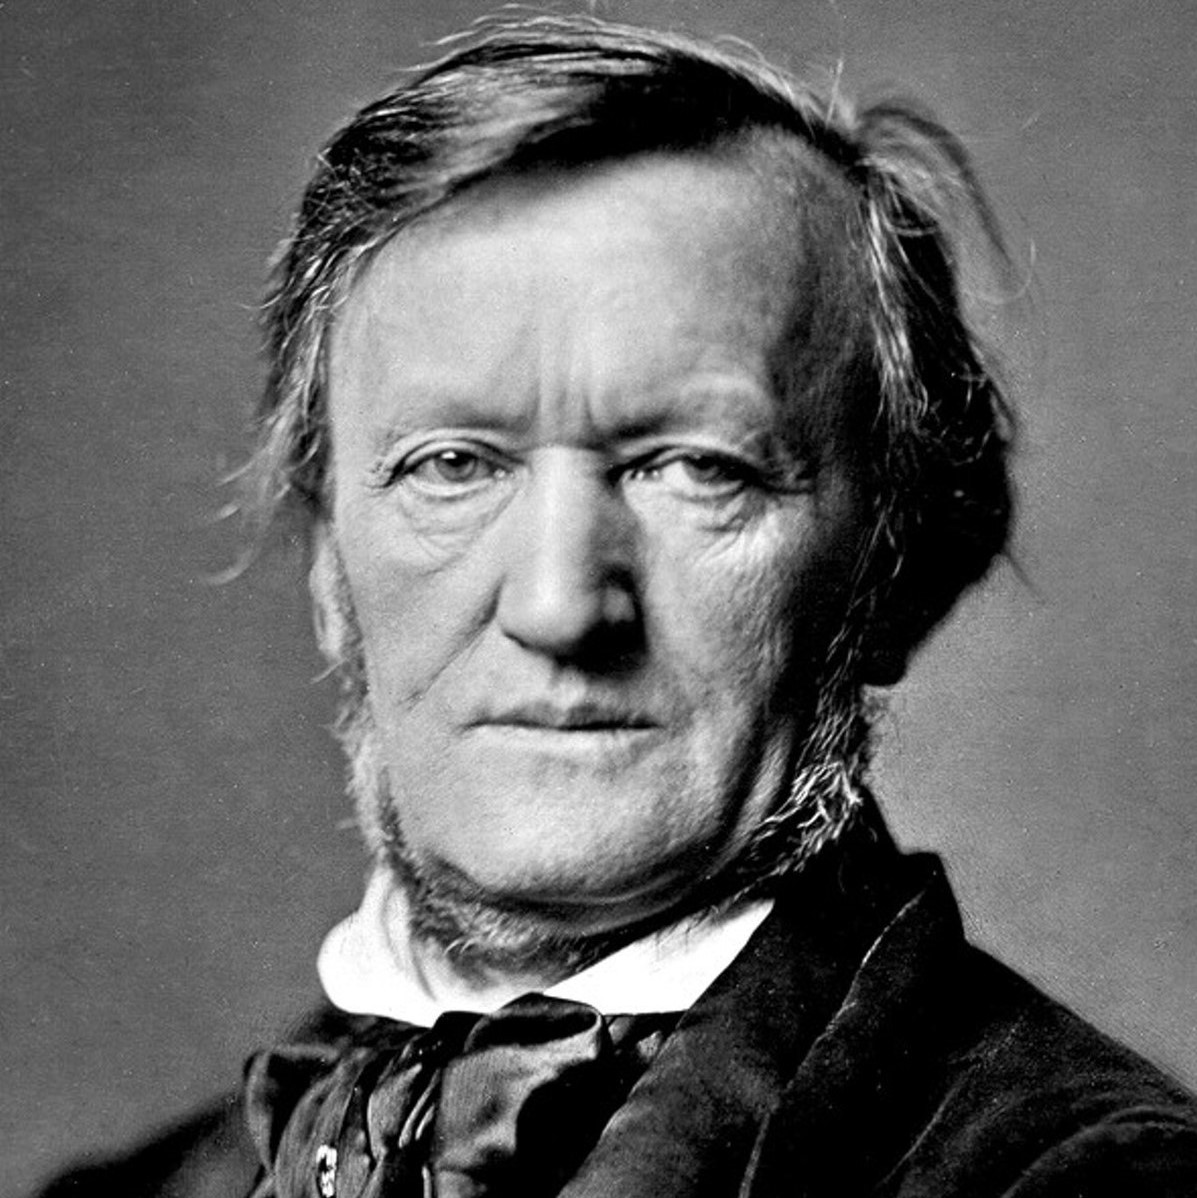
\includegraphics[width=0.22\textwidth]{Richard_Wagner.jpg}			
			\caption*{Richard Wagner\\(1813--1883)}	}
		\end{wrapfigure}
		El periodo de la historia de la música predominante en el siglo XIX, comúnmente llamado Romanticismo, culminó con los dramas musicales de Richard Wagner, en los que todos los elementos de la obra estaban detalladamente estudiados por el compositor. A este concepto lo llamaba \emph{Gesamtkunstwerk} (<<obra de arte total>>\footnote{Richard Wagner, \emph{Oper und Drama}, 1851.}), ya que creía poseer la responsabilidad de reunir todas las artes en una misma obra. Wagner se aseguraba personalmente de que en sus óperas las artes escénicas, musicales, poéticas y visuales se combinaran entre sí a la perfección.
	
		La idea del \emph{Gesamtkunstwerk} la desarrolló alrededor de 1850, y la plasmó en su totalidad en su ciclo de cuatro óperas \emph{Der Ring des Nibelungen}, estrenado el 16 de agosto de 1876. Wagner controló y creó cada aspecto de la tetralogía, desde la música hasta el libreto, el vestuario y la escenografía. Incluso mandó crear su propia sala de conciertos en Bayreuth, el \emph{Festspielhaus}, para que el escenario se adecuara a sus ideas sobre el pensamiento y la cultura musical.
	
		Así, a ojos de compositores posteriores, Wagner había agotado todas las posibilidades de la música tonal, y quizás ya había comenzado el viraje hacia el predominio de la disonancia con su abundante uso del cromatismo, como en el famoso primer acorde del drama musical \emph{Tristan und Isolde} (1865). Consta de las notas Fa, Si, $\text{Re\#}$ y $\text{Sol\#}$, y sus intervalos desde el Fa son una cuarta aumentada, una sexta aumentada y una novena aumentada.
		
		Siguiendo la concepción del progreso como un camino ascendente, el paso siguiente para la composición musical debía consistir en deshacerse progresivamente de la tonalidad y desarrollar la <<emancipación de la disonancia>>\footnote{Arnold Schoenberg, \emph{Composition with twelve tones}, en \emph{Style and Idea}, 1950.}. Así fue como Arnold Schoenberg ideó sus teorías del pensamiento musical, y éstas dieron paso a la creación de la atonalidad. \cite{kinney}
	
	\section{Hacia el atonalismo de Schoenberg}
		Fuertemente influido por Richard Wagner y Johannes Brahms desde su adolescencia, Schoenberg comenzó componiendo al estilo posromántico de su época, llevando el cromatismo y la orquestación hasta el extremo. Sin embargo, y no espontáneamente, empezó a buscar en sus composiciones que cada sonido tuviera valor por sí mismo, un valor independiente de su funcionalidad tonal. 
		
		\begin{wrapfigure}{L}{0.3\textwidth}
			\captionsetup{justification=centering, font=footnotesize}
			\centering{
				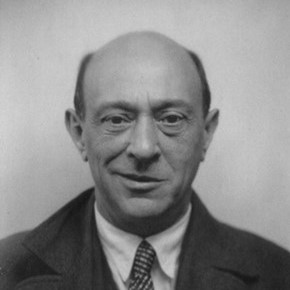
\includegraphics[width=0.22\textwidth]{Arnold_Schoenberg.jpg}			
				\caption*{Arnold Schoenberg\\(1874--1951)}	}
		\end{wrapfigure}
		Para él, la música no estaba intrínsecamente dirigida a una tónica. En las progresiones, lo importante era el paso de un acorde a otro, y no hacia dónde se dirigían éstos. Además, él opinaba que se debían poder utilizar las notas de los modos eclesiásticos libremente, por lo que consideraba las notas no diatónicas tan válidas como las diatónicas. Esto hacía imposible distinguir unas de otras, no pudiendo identificar apenas la tónica. De esta, y de otras muchas formas, Schoenberg conseguía que la jerarquía tonal quedara desestabilizada. \cite{kinney}
		
		De esta época es su primera obra importante, \emph{Verklärte Nacht} (<<Noche transfigurada>>), Op. 4. Compuesto en 1899, este sexteto de cuerdas está inspirado por el poema homónimo de Richard Dehmel. La música, según su autor, expresa el paseo de un hombre y una mujer en medio del abrazo de la naturaleza.  Aunque en la obra aún prevalece la armonía tradicional basada en acordes, Schoenberg sitúa al oyente en un terreno de indefinición tonal, no sólo en el plano armónico sino también en el melódico. Además, hace uso del acorde de novena invertido, inexistente hasta entonces y, por tanto, rechazado por la crítica. \cite{diaz}
				
		Tras pasar por la etapa tonal posromántica, y debido a su convicción en la irrevocabilidad de la evolución de la música hacia el cromatismo total \cite{delgado}, en 1908 Schoenberg se desligó de la tonalidad completamente con el ciclo de canciones \emph{Das Buch der Hängenden Gärten}. A partir de entonces se dedicó a componer fragmentos muy breves cuya estructura era definida por motivos y no por la armonía, como solía ocurrir en formas musicales anteriores\footnote{La forma sonata es el ejemplo más destacado de estructura basada en la armonía.}. A este periodo en sus composiciones se le llama \emph{atonalidad libre}, aunque cabe destacar que Schoenberg rechazaba fervientemente este término:
		
		\begin{quote}
			\emph{La expresión “música atonal” es de lo más desafortunada -- es como llamar a volar “el arte de no caer” o nadar “el arte de no ahogarse”.}\footnote{A. Schoenberg, \emph{Hauer's Theories}, en \emph{Style and Idea}, 1923.}
		\end{quote}
				
		A este periodo -- es de 1912 -- pertenece también su famoso ciclo de canciones \emph{Pierrot Lunaire}, Op. 21. Su nombre completo es ``Tres veces siete poemas de Pierrot Lunaire de Albert Giraud'', ya que está dividida en 3 grupos de 7 canciones cada uno, cuyos textos son una selección de 21 poemas del ciclo homónimo de Albert Giraud. 
		
		Se encuentran en ella abundantes referencias al número 7: Schoenberg hace un uso extensivo de motivos de 7 notas a lo largo de la obra, mientras que el conjunto musical que la interpreta, incluyendo al director, consta de 7 miembros. De hecho, a este conjunto de instrumentos -- flauta, clarinete, violín, violonchelo, piano y cantante -- se le ha dado el nombre de \textit{ensemble Pierrot} en su honor. 
		
		Otros números importantes en la obra son el 3 y el 13. Cada poema consta de 13 líneas, mientras que la primera línea de cada poema aparece 3 veces: en las líneas 1, 7 y 13.
		
		En esta obra no sólo hay una ausencia total de relaciones tonales, sino que el tratamiento vocal evita también cualquier relación estética con las técnicas tradicionales: es un \emph{Sprechgesang}, un canto hablado. De hecho, Schoenberg se refiere a estas piezas no como canciones, sino como melodramas. \cite{diaz}
		
	\section{El surgimiento de un sistema}
		Schoenberg no estaba aún satisfecho con su técnica compositiva, ya que admiraba las obras extensas de los músicos románticos y pensaba que su atonalidad no podía sostener una obra de gran envergadura. Es decir, necesitaba un hilo conductor mejor que los motivos para poder componer obras atonales más largas.
		
		Además, por aquella época sufrió una crisis en muchos aspectos de su vida. En lo personal, su mujer Matilde Zemlinsky acababa de abandonarlo por otro hombre, aunque posteriormente volvería junto al compositor. Y, en lo profesional, sus obras no eran del gusto del público, por lo que no contaba con suficiente dinero para mantener a su familia. Todas estas circunstancias, unidas al desarrollo de la Primera Guerra Mundial, no le permitieron componer apenas entre 1914 y 1923.
		
		Tras el final de la guerra, en 1919, Schoenberg fundó la Sociedad para Interpretaciones Musicales Privadas junto a sus discípulos y amigos Alban Berg y Anton Webern. Schoenberg, Berg y Webern se autodenominaron la Segunda Escuela de Viena en honor al grupo de compositores del siglo XVIII Haydn, Mozart y Beethoven, quienes formaban la Primera Escuela de Viena.\footnote{Las carreras compositivas de Berg y Webern se desarrollarán en el apartado \ref{berweb}.}
		
		En la Sociedad para Interpretaciones Musicales Privadas se presentaban músicas contemporáneas en circunstancias que favorecieran su adecuada apreciación. Así se evitaba que dichas obras, al no ser entendidas por el público, fueran inmediatamente rechazadas. Las obras de compositores como Mahler, Debussy, Bartók, Ravel, Strauss y Stravinsky fueron incluidas en los programas de conciertos organizados por la Sociedad.
		
		En este contexto Schoenberg pudo reflexionar sobre sus técnicas compositivas, y al fin publicó en 1923 su ensayo \emph{Método de composición con doce sonidos}, donde se describían por primera vez los axiomas del dodecafonismo: la solución al problema de la atonalidad libre que le había estado atormentando durante una década.
		
		Su primera obra íntegramente dodecafónica, publicada también en 1923, es la Suite para piano Op. 25. Es la pieza más temprana en la que Schoenberg usa series dodecafónicas en cada uno de los movimientos. En dos obras anteriores a ella usa series dodecafónicas, pero en movimientos aislados: la Op. 23, \emph{5 Stücke} (1920--23), en el movimiento de Waltz final; y su \emph{Serenata}, Op. 24, en su Soneto central.
		
		Las series utilizadas en la Suite Op. 25 servirán de ejemplo en este texto, y su tercer movimiento, Musette, será estudiado y analizado en el apartado \ref{musette} con el fin de entender una obra dodecafónica en toda su extensión.